\section{Experiments}
In this section, we aim to answer the following two questions: 1) Are the existing representative methods capable of solving the tasks in \algo? 2) Within each paradigm, will the differentiable simulator help in completing the tasks?

To investigate these two questions, we benchmark eight representative methods of deformable object manipulation, covering planning, imitation learning, and reinforcement learning. Each paradigm has different assumptions and requirements for input knowledge. We summarize the baseline methods and the relevant information in Table \ref{tab:deformable_manipulation_methods}. 

\subsection{Experimental Setup}

\begin{table}[t]
    \centering
    \fontsize{8}{8}\selectfont
    \begin{tabular}{c c c c c c c c c}
\toprule
Paradigms &\multicolumn{3}{c}{Reinforcement Learning} 
& \multicolumn{2}{c}{Imitation Learning}
& \multicolumn{3}{c}{Planning}
\\
\cmidrule(lr){1-1}
\cmidrule(lr){2-4}
\cmidrule(lr){5-6}
\cmidrule(lr){7-9}
Methods & PPO & SHAC & APG & Transporter & ILD & CEM-MPC & diff-MPC & diff-CEM-MPC  \\
\cmidrule(lr){1-1}
\cmidrule(lr){2-4}
\cmidrule(lr){5-6}
\cmidrule(lr){7-9}
 
\# expert demos &
\NA & \NA & \NA &
10 & 1 &
\NA & \NA  & \NA
\\  [0.5em]
Reward function  & \cmark & \cmark & \cmark & \NA & \NA & \cmark & \cmark  & \cmark   \\
\cmidrule(lr){1-1}
\cmidrule(lr){2-4}
\cmidrule(lr){5-6}
\cmidrule(lr){7-9}

 Differentiability & \xmark & \cmark & \cmark & \xmark & \cmark & \xmark & \cmark & \cmark \\  
\bottomrule
    \end{tabular}
    \caption{\textbf{Methods on Deformable Object Manipulation with respect to different setups.} 
    }
\label{tab:deformable_manipulation_methods}
\end{table}   




\textbf{Reward function} For each task, the goal is specified by the desired final positions of the set of particles, $g$, representing the deformable object. In this setup, the reward can be intuitively defined by how well the current object particles match with those of the goal. Hence, we define the ground-truth reward as
$r_{\text{gt}}(s, a) = \exp(- \lambda D(s',g))$,
where $s'$ is the next state resulted from $a$ at the current state $s$, and $ D (s,g)$ is a non-negative distance measure between the positions of the object's particles $s$ and those of the goal $g$.

However, using the ground-truth reward alone is inefficient for learning.
The robot's end-effector can only change the current object pose by contacting it. Therefore, to most efficiently manipulate the object to the desired configuration, we add an auxiliary reward to encourage the robot to contact the object. We define the auxiliary reward as
$r_{\text{aux}}(s, a) = \exp(- L_2(s, a))$,
where $L_2(s, a)$ measures the $L2$ distance between the end-effector and the object. During training, we use the sum of the ground-truth and auxiliary reward functions $r_{\text{gt}} + r_{\text{aux}}$, and during evaluation, we only use the ground-truth reward $r_{\text{gt}}$.

\subsection{Reinforcement Learning}
\begin{table}[t]
    \centering
    \begin{tabular}{cccc}
    \hspace{-5mm}
         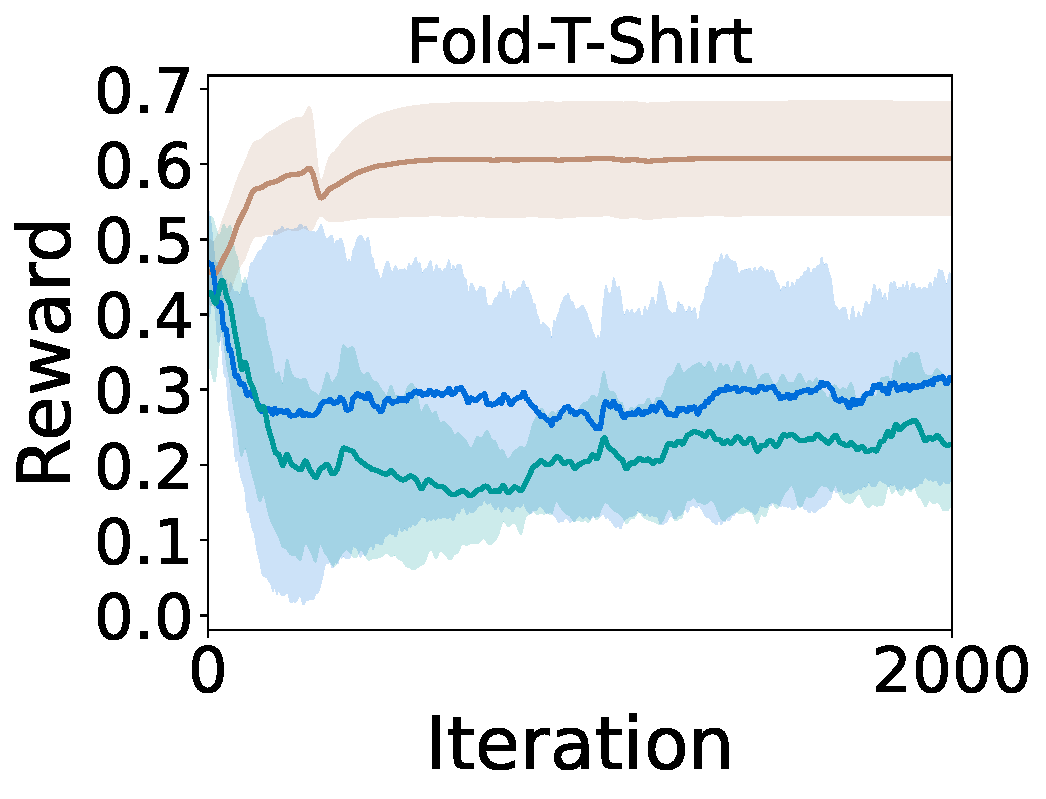
\includegraphics[width=0.23\textwidth]{iclr2023/figs/rl_training_curve/fold_tshirt.pdf}
         &
        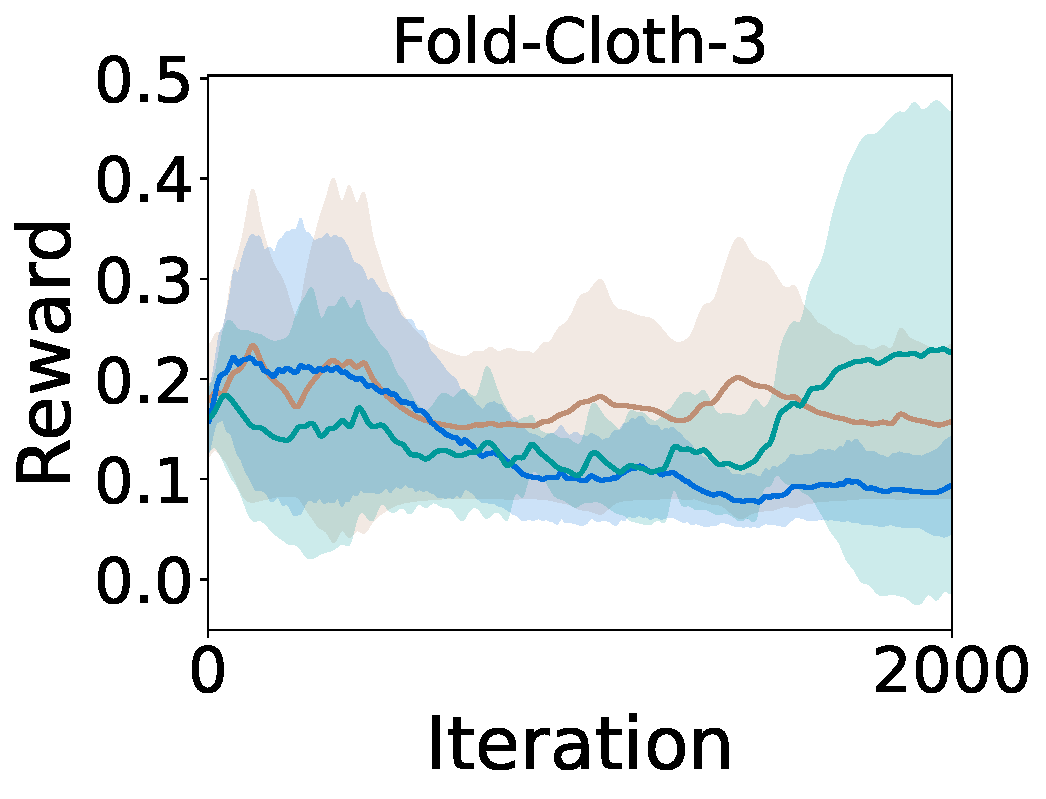
\includegraphics[width=0.23\textwidth]{iclr2023/figs/rl_training_curve/fold_cloth3.pdf}
         &
        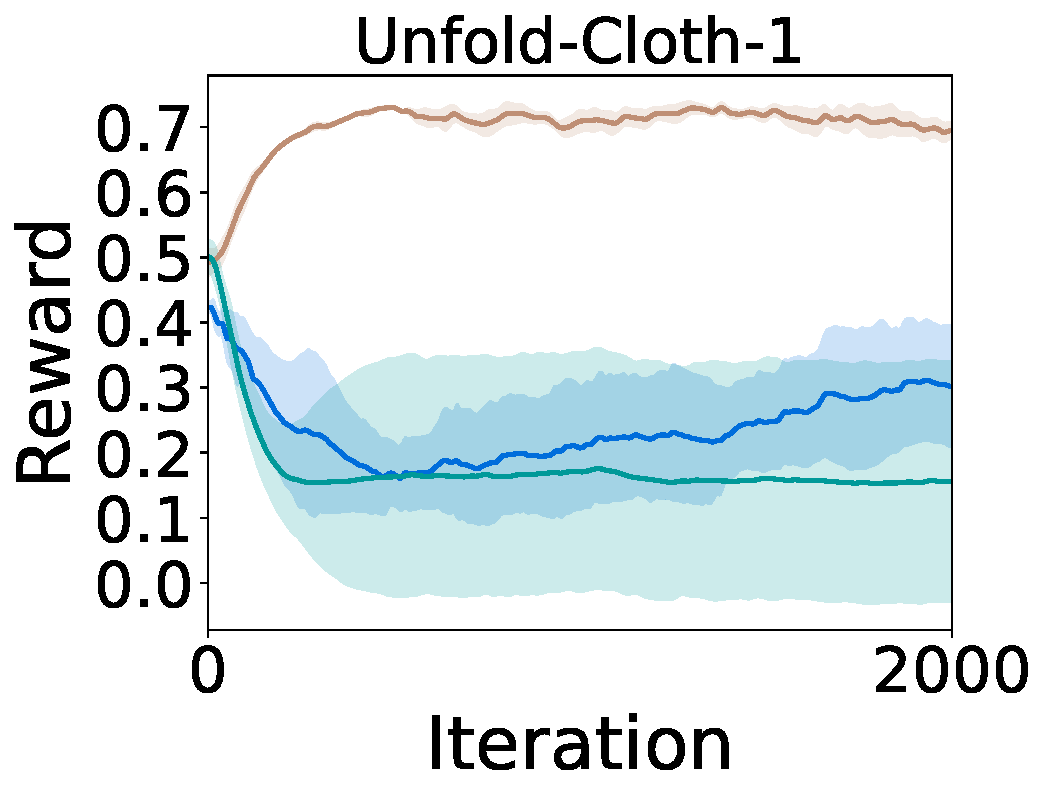
\includegraphics[width=0.23\textwidth]{iclr2023/figs/rl_training_curve/unfold_cloth1.pdf}
         &
        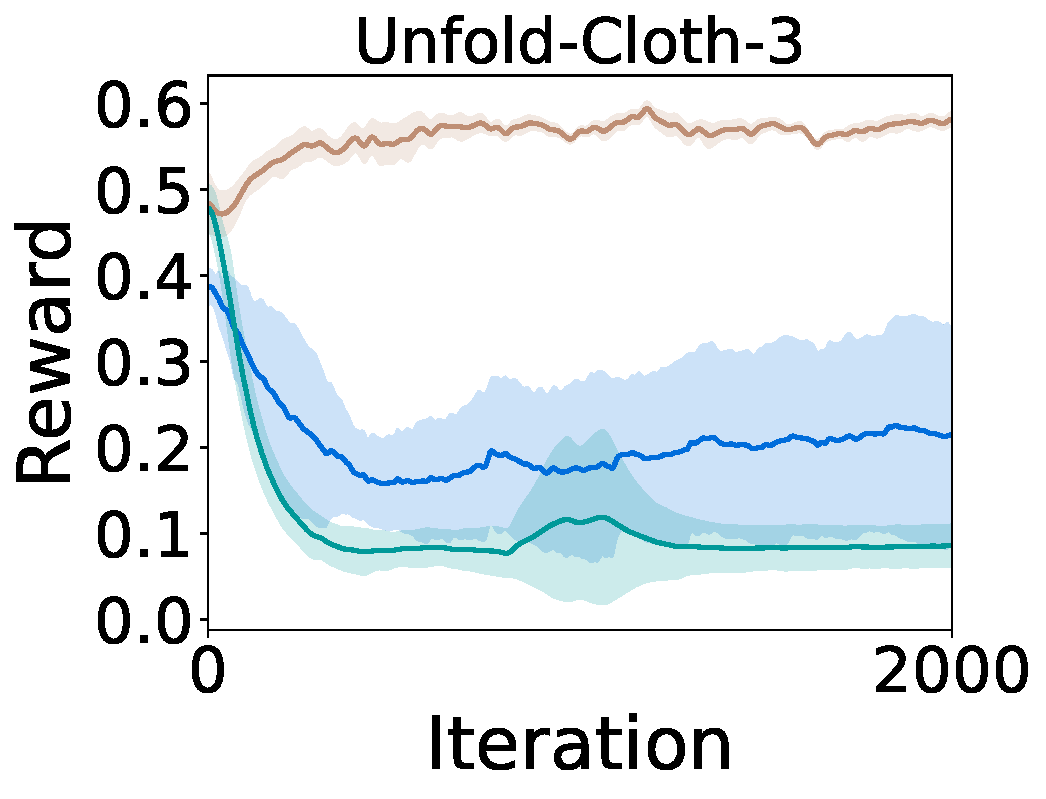
\includegraphics[width=0.23\textwidth]{iclr2023/figs/rl_training_curve/unfold_cloth3.pdf}
         \\
             \hspace{-5mm}
        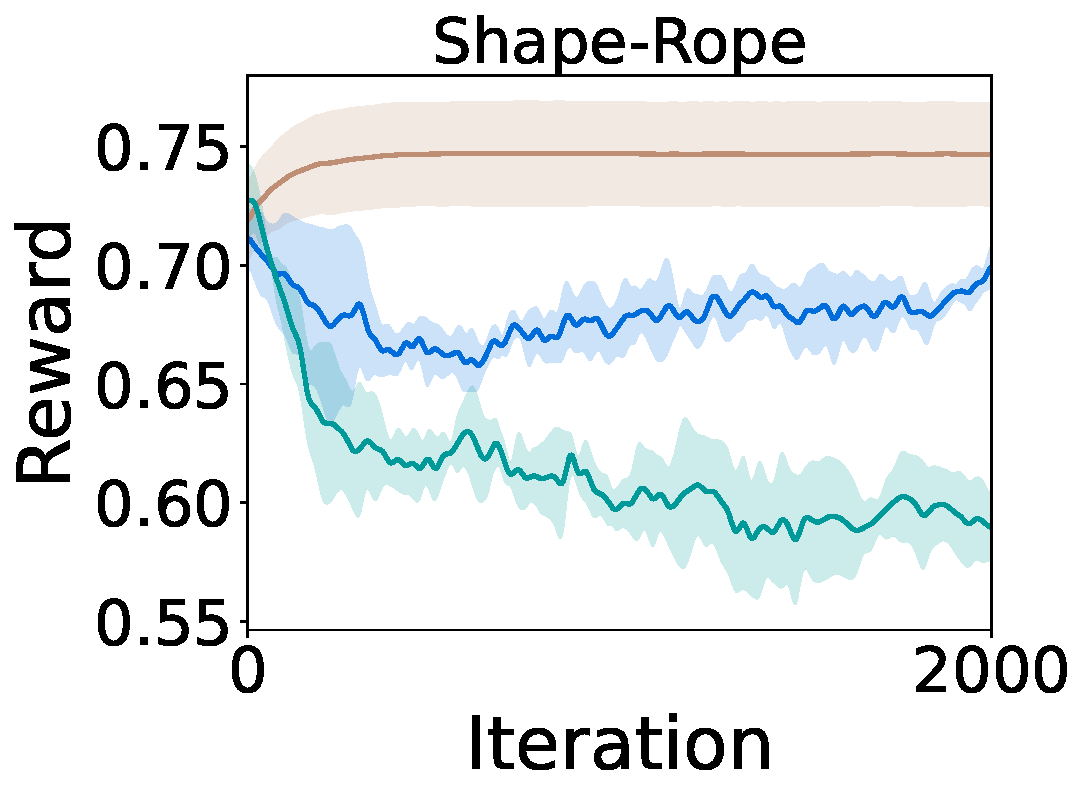
\includegraphics[width=0.23\textwidth]{iclr2023/figs/rl_training_curve/shape_rope.pdf}
         &
        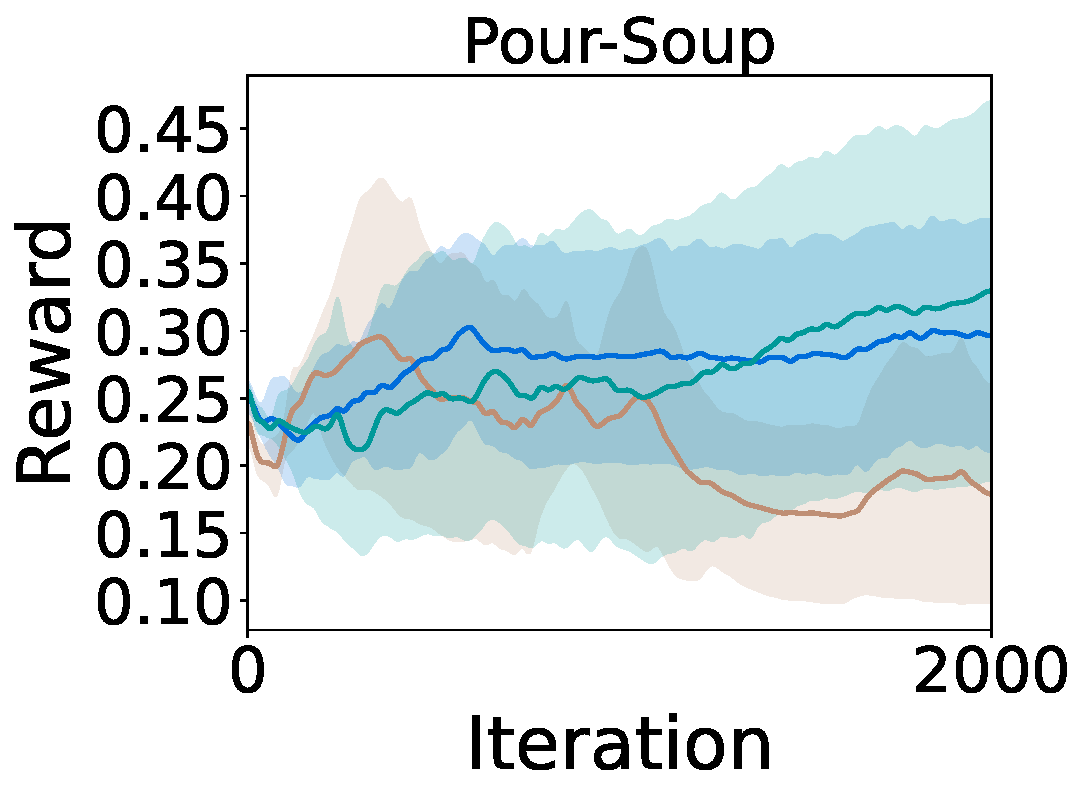
\includegraphics[width=0.23\textwidth]{iclr2023/figs/rl_training_curve/pour_soup.pdf}
         &
        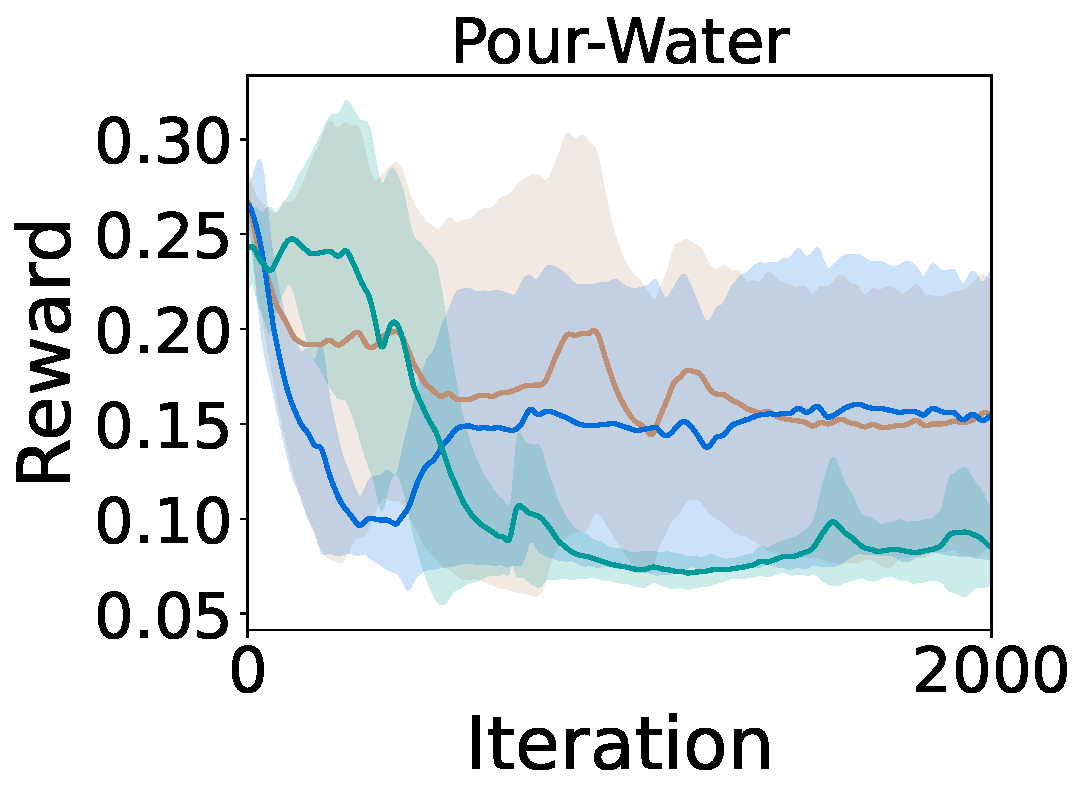
\includegraphics[width=0.23\textwidth]{iclr2023/figs/rl_training_curve/pour_water.pdf}
         &       
         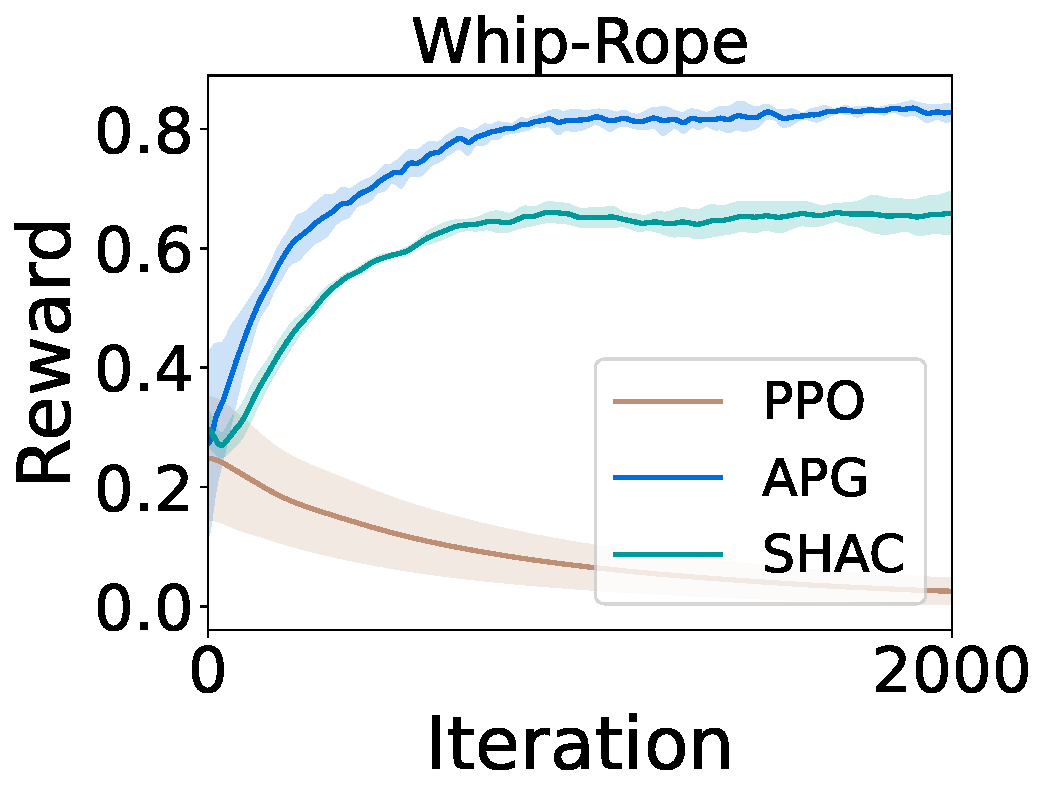
\includegraphics[width=0.23\textwidth]{iclr2023/figs/rl_training_curve/whip_rope.pdf}

    \end{tabular}
    \captionof{figure}{\textbf{Learning curves of three benchmarked RL algorithms: PPO, APG, and SHAC.} The y-axis shows the episode reward, scaled from 0 to 1, with larger values being closer to the goal state. The x-axis is the number of training iterations. All methods are trained in the same number of batched environments. We report the mean and variance of the performance for 5 seeds and each seed has 20 rollouts with different initializations. We refer the readers to Table \ref{table:RL_results} for the numerical results in the appendix.
    }
    \label{tab:rl_learning_curves}
\end{table}
\textbf{Methods.} We benchmark PPO ~\citep{PPO}, SHAC ~\citep{SHAC}, and APG ~\citep{Brax} as the representative RL methods. PPO is a widely used model-free non-differentiable RL method with competitive performance, while SHAC and APG are the two latest RL methods that utilize the differentiable simulator. The computation graph of SHAC is illustrated in Figure \ref{fig:cg_rl}. By comparing the performance of the \algo\ tasks across these three methods, we aim to further study the benefits and limitations of applying the differentiable physics to RL.

\textbf{Overall Performance.}
The learning curves of RL methods are shown in Figure \ref{tab:rl_learning_curves}.
The performance difference between PPO and the differentiable RL methods shows opposite trends in the high-level macro-action-based and local-level control tasks. To our surprise, for most of the short-horizon macro-action-based tasks, PPO performs consistently better than the differentiable RL methods. This seems to contradict the experiment results of SHAC~\citep{SHAC}, which shows stronger performance than PPO in its own simulator on a wide range of context-rich MuJoCo tasks.
However, for long-horizon tasks with low-level controls, the differentiable RL methods, especially APG, outperform PPO by a large margin.

\textbf{Main Challenge for the differentiable-physics-based RL methods: Exploration.}
We argue that, on high-level macro-action-based tasks, the main limiting factor of the performance of differentiable-physics-based RL is the lack of exploration during training.
The need to balance this trade-off is exaggerated by the enormous DoFs and the complex dynamics unique to the DOM tasks. Especially for the high-level macro-action-based tasks, their non-smooth/discontinuous/non-convex optimization landscape necessitates using a good exploration strategy. 
However, the existing differentiable-physics-based RL methods rely exclusively on the simulation gradient to optimize the policy. They are not entropy regularized; hence, they may quickly collapse to the local optimal.
Without explicit exploration, the differentiable-physics-based RL methods fail to reach the near-optimal state using the simulation gradients alone. Taking Fold-Cloth-3 as an example, if the randomly initialized policy never touches the cloth, the local simulation gradients cannot guide the agent to touch the cloth since the rewards and, consequently, the gradients for all not-in-contact actions are zero. 

\textbf{Differentiable-physics-based RL are sensitive to the Optimization Landscape.} Differentiable-physics-based RL can largely improve the performance of some low-level control tasks if the optimization landscape is smooth and convex. Taking Whip-Rope as an example, the optimal low-level control sequence is a smooth motion trajectory that lies on a relatively smooth and well-behaved plane for the gradient-based methods. This explains why APG outperforms the non-differentiable-physics-based PPO by a large margin. 

\subsection{Imitation Learning}

\begin{table}[t]
\centering
\fontsize{7.5}{7.5}\selectfont
\begin{tabular}{lccccccc}
\toprule
 &  & \multicolumn{3}{c}{Imitation Learning} &  \multicolumn{3}{c}{Planning}\\
 \cmidrule(lr){1-2}
 \cmidrule(lr){3-5} 
\cmidrule(lr){6-8} 
Task Type   
& Task & Transporter & ILD & Expert
 & CEM-MPC & Diff-MPC & Diff-CEM-MPC\\
\cmidrule(lr){1-2}
\cmidrule(lr){3-5} 
\cmidrule(lr){6-8} 
\multirow{6}{*}{High-level} 

& Fold-Cloth-1 

& 0.19$\pm$0.04 & 0.76$\pm$0.04 & 0.91$\pm$0.00

&0.74$\pm$0.07 & 0.29$\pm$0.07 &0.80$\pm$0.04 
\\


& Fold-Cloth-3 

& 0.40$\pm$0.05 &   0.82$\pm$0.05 & 0.89$\pm$0.00

& 0.62$\pm$0.08 & 0.14$\pm$0.02 & 0.66$\pm$0.07 

\\


& Fold-T-shirt 

& 0.46$\pm$0.02 &  0.59$\pm$0.11 & 0.85$\pm$0.00 

& 0.58$\pm$0.04 & 0.29$\pm$0.06 & 0.66$\pm$0.01

\\


& Unfold-Cloth-1 

 &0.48$\pm$0.01 & 0.64$\pm$0.03 & 0.87$\pm$0.00
 
 &  0.57$\pm$0.04 & 0.30$\pm$0.05 & 0.67$\pm$0.02  


\\


&Unfold-Cloth-3 

 & 0.30$\pm$0.00 & 0.52$\pm$0.02 &0.87$\pm$0.00
 
 & 0.57$\pm$0.01 & 0.26$\pm$0.04 & 0.58$\pm$0.01 

\\

& Push-Rope

&  0.70$\pm$0.00 & 0.76$\pm$0.02 & 0.93$\pm$0.00 

& 0.71$\pm$0.01 & 0.70$\pm$0.01 &0.71$\pm$0.01  

\\
\cmidrule(lr){1-2}
\cmidrule(lr){3-5} 
\cmidrule(lr){6-8}
\multirow{3}{*}{Low-level}

&Whip-Rope 

& \NA  &0.70$\pm$0.06 & 1.00$\pm$ 0.00
& 0.34$\pm$0.01 & 0.37$\pm$0.00&0.33$\pm$0.01
\\


&Pour-Water 

& \NA &0.32$\pm$0.03 & 0.91$\pm$ 0.06

& 0.58$\pm$0.01 & 0.30$\pm$0.00 & 0.58$\pm$0.01
\\

& Pour-Soup  

& \NA & 0.42$\pm$0.12 & 0.85$\pm$ 0.00

& 0.56$\pm$0.01  & 0.44$\pm$0.00 & 0.55$\pm$0.02 
\\
\bottomrule
\end{tabular}
\caption{\small \textbf{Task performance for the planning and imitation learning methods.} We report the mean and standard error for the policy/control sequences evaluated under 20 seeds.}
\label{table:planning_il}
\end{table}


\textbf{Methods.}
We benchmark Transporter ~\citep{transporter} and ILD ~\citep{ILD} as the two representative Imitation Learning DOM methods. Transporter is a popular DOM method that is well-known for its simple implementation and competitive performance. We use particles as input to evaluate the performance of Transporter in our experiment for a fair comparison. The original implementation of Transporter uses RGBD as input. We refer the readers to the Appendix \secref{sec:transporter} for the performance of the Transporter with RGB channels. ILD is the latest differentiable-physics-based IL method; it utilizes the simulation gradients to reduce the required number of expert demonstrations and to improve performance. Note that since Transporter abstracts its action space to \textit{pick-and-place} actions to simplify the learning, it cannot be extended to the low-level control tasks. Our comparison of the IL methods will first focus on the high-level macro-action-based tasks, then we will analyze the performance of ILD with the expert.

\textbf{Overall performance} For the high-level macro-action-based tasks, ILD outperforms Transporter by a large margin for all tasks. For example, ILD outperforms Transporter in Fold-Cloth-1, Fold-Cloth-3, and Unfold-Cloth-1. We highlight that this significant performance gain is achieved by using a much smaller number of expert demonstrations. We attribute this improvement to the additional information provided by the simulation gradients, where now ILD can reason over the ground-truth dynamics to bring the trajectory closer to the expert, at least locally. As illustrated in Figure \ref{fig:computation_graph}, the gradients used to optimize each action comes from the globally optimal expert demonstrations 1) at the current step and 2) in all the steps after. In contrast, the gradients used in SHAC only count the reward at the current step. The differentiable RL faces the challenge of exploding/vanishing gradients and lack of exploration. Differentiable IL alleviates these problems by having step-wise, globally optimal guidance from expert demonstrations.

\textbf{Challenge for ILD: Unbalanced State Representations.} ILD does not perform well on tasks like Pour-Water and Pour-Soup with unbalanced state representations, for example, $1000 \times 3$ features of particles and 6 gripper states. The learned signals from the particles overwhelm the signals from the gripper states. Therefore, ILD cannot learn useful strategies with unbalanced learning signals. Softgym \citep{softgym} also concurs with the results that policies with reduced state representation perform better than those with the full state. A more representative representation of the states needs to be considered and we leave it for future study.

\begin{figure}[t]
\centering\subcaptionbox{SHAC.\label{fig:cg_rl}}{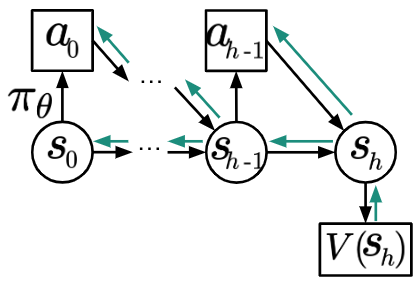
\includegraphics[height=0.17\columnwidth]{iclr2023/figs/computation_graph/RL.png}} \hfill
\subcaptionbox{ILD.\label{fig:cg_il}}{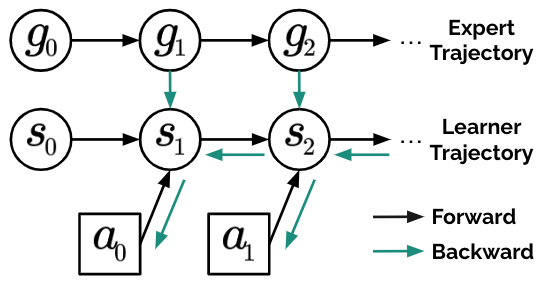
\includegraphics[height=0.17\columnwidth]{iclr2023/figs/computation_graph/IM.png}}
 \hfill
\subcaptionbox{Diff CEM-MPC.\label{fig:cg_planning}}{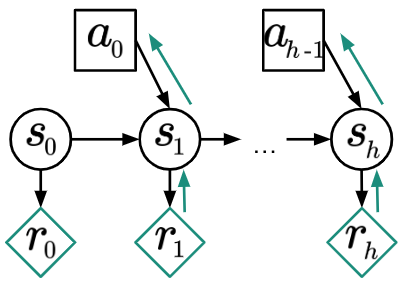
\includegraphics[height=0.17\columnwidth]{iclr2023/figs/computation_graph/Planning.png}} \hfill
\caption{
\textbf{Computation graphs for the differentiable algorithms.} We use SHAC, ILD, and Diff CEM-MPC to represent the differentiable algorithms for planning, RL, and IL respectively. The black/green arrows correspond to the forward/backward propagation respectively.
}
\vspace{-3mm}
\label{fig:computation_graph}
\end{figure}

In conclusion, differentiable methods can optimize the policies efficiently if the optimization landscape is well-behaved. For tasks that require tremendous explorations or with sparse rewards, gradient-based methods suffer severely from the local minima and gradient instability issues. 

\subsection{Planning}
\textbf{Methods.}
We benchmark the classic CEM-MPC ~\citep{Richards2005RobustCM} as a representative random shooting method that uses a gradient-free method to optimize the action sequences for the highest final reward. To study the effect of using differentiable physics, we implement two versions of differentiable MPC. The basic computation graph for both is illustrated in Figure \ref{fig:cg_planning}. In particular, both differentiable MPC baselines maximize the immediate reward of each action using differentiable physics. The difference lies in the initial action sequences: diff-MPC is initialized with a random action sequence, while diff-CEM-MPC with an action sequence optimized by CEM-MPC.

\textbf{Overall Performance.} The diff-CEM-MPC performs consistently better than or on par with CEM-MPC, while Diff-MPC fails to plan any reasonable control sequences for most of the tasks. 

\textbf{Simulation Gradients as Additional Optimization Signals.} The vastly different performance between the two versions of the differentiable baselines brings us insights into how differentiable physics helps in planning. Simulation gradients provide additional signals in the direction to optimize the actions, thereby reducing the sample complexity. However, similar to any gradient-based optimization methods, differentiable planning methods are sensitive to the non-convex/non-smooth optimization landscape and face a major limitation of being stuck at the local optimal solution. DOM's enormous DoFs of DOM and complex dynamics exacerbate these challenges for the differentiable DOM planning methods. 

\textbf{Differentiable Planning needs Good Initialization.} We attribute the poor performance of Diff-MPC to its random control sequence initialization. In particular,  this control sequence may significantly deviate from the optimal one over the non-smooth/non-convex landscape, such that the simulation gradients alone cannot bring the control sequence back to the optimal. In contrast, Diff-CEM-MPC is initialized with the optimized control sequence by CEM-MPC, which relies on iterative sampling followed by elite selection to escape the local optimality. Hence, the control sequence fed into the differentiable step is already sufficiently close to the globally optimal solution. The simulation gradients help diff-CEM-MPC to optimize the action sequences further locally, which explains the performance gain. 

To summarize, the differentiable simulator can further optimize the near-optimal control sequences locally with much low sample complexity. Yet, its performance critically relies on a good initialization and a locally smooth optimization landscape.

\begin{figure}[t]
    \centering
    \begin{tabular}{cc}
    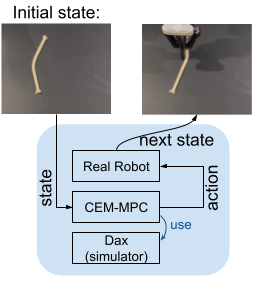
\includegraphics[height=0.285\linewidth]{iclr2023/figs/sim2real/sim2real-system.png}
    & 
    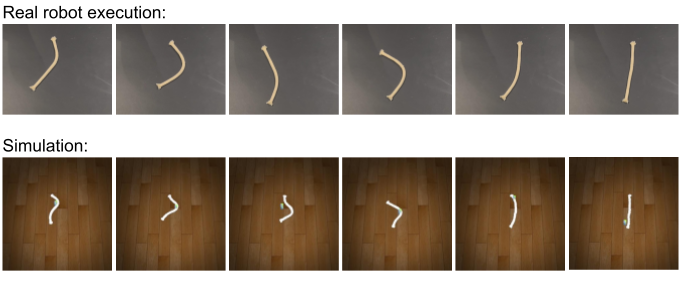
\includegraphics[height=0.285\linewidth]{iclr2023/figs/sim2real/sim2real-traj.png}
    \\
    (a) & (b)
    \end{tabular}
    \caption{\textbf{We deploy CEM-MPC in a Push-Rope task to straighten the rope in 6 steps on a real robot}.
    (a) The system structure. CEM-MPC uses our \simulator\ simulator as the predictive model. Given the current state estimated from a point cloud image, CEM-MPC plans the best action to be executed by the robot.
    (b) The states after each of the 6 pushes. We compare the dynamics in reality and in simulation. Top: state trajectory in a real robot experiment. Bottom: the next state predicted by \simulator\ given the estimated current state and the corresponding planned action.}
    \label{fig:sim2real_states}
    \vspace{-3mm}
\end{figure}

\subsection{Sim-2-Real Gap}
Granted that the physical engine of \simulator\ is built upon a state-of-the-art simulation method, the fidelity and correctness still need to be tested.
To testify to the correctness of our simulated dynamics to real-world physics, we carry out a real robot experiment on a Kinova Gen 3 robot.
We deploy CEM-MPC with \simulator\ as the predictor model to a Push-Rope task, as shown in Figure \ref{fig:sim2real_states}.
Our study finds that the resultant state trajectories are similar in simulation and in reality.
This validates the fidelity of the tasks implemented based on our engine, and the performance of the DOM methods in our simulator provides hints about their performance on the real robot.
We refer the reader to the appendix for details. 
In addition, the differentiability of \simulator\ enables system identification that can reduce the sim-2-real gap \citep{le2021differentiable, murthy2021gradsim}.
We can get an error term by comparing the observations in simulation and in reality; by differentiating this error with respect to the simulator parameters, we get gradients for parameter tuning.





